\documentclass[12pt]{article}

\addtocounter{secnumdepth}{1}

\usepackage[utf8]{inputenc}
\usepackage[margin=1.0in]{geometry}

\usepackage{enumitem}
\usepackage{pdfpages}
\usepackage{graphicx}
\usepackage[export]{adjustbox}
\usepackage{float}
\usepackage[tablegrid,nochapter]{vhistory}
\usepackage[parfill]{parskip}

\usepackage{listings}
\usepackage{color}

\definecolor{codegreen}{rgb}{0,0.6,0}
\definecolor{codegray}{rgb}{0.5,0.5,0.5}
\definecolor{codepurple}{rgb}{0.58,0,0.82}
\definecolor{backcolour}{rgb}{0.95,0.95,0.92}
 
\lstdefinestyle{cstyle}{
    backgroundcolor=\color{backcolour},
    commentstyle=\color{codegreen},
    keywordstyle=\color{magenta},
    numberstyle=\tiny\color{codegray},
    stringstyle=\color{codepurple},
    basicstyle=\footnotesize,
    breakatwhitespace=false,
    breaklines=true,
    captionpos=b,
    keepspaces=true,
    numbers=left,
    numbersep=5pt,
    showspaces=false,
    showstringspaces=false,
    showtabs=false,
    tabsize=2
}
 
\lstset{style=cstyle}

\newlist{purposelist}{enumerate}{1}
\setlist[purposelist]{label=\thesubsection.\arabic*.,resume}

\newlist{doclist}{enumerate}{1}
\setlist[doclist]{label=\thesubsection.\arabic*.,resume}

\newlist{equiplist}{enumerate}{1}
\setlist[equiplist]{label=\thesubsection.\arabic*.,resume}

\newlist{deflist}{enumerate}{1}
\setlist[deflist]{label=\thesubsection.\arabic*.,resume}

\begin{document}

\begin{titlepage}
	\raggedright
	\topskip0pt
	\vspace*{\fill}
	\textbf{TITLE:} Study of the Balloon Catheterization Microcontroller \\
	\vspace{2cm}
	\textbf{DATE:} April 28, 2019 \\
	\vspace{2cm}
	\textbf{PRINCIPAL INVESTIGATOR:} Nam Tran \\
	\vspace{2cm}
	\textbf{PRINCIPAL INVESTIGATOR SIGNATURE:} \\
	\vspace{2cm}
	\textbf{INVESTIGATORS:} N/A \\
	\vspace*{\fill}
\end{titlepage}

\section{Overview}
\subsection{Purpose}
The primary focus of this study is to test and verify the ESP32 microcontroller's functionality as used in the Balloon-Catheterization capstone project. This is not a materials justification, but rather an assurance that the device selected will not cause bugs.

\subsection{Scope/Application}
The ESP32 microcontroller used in this study serves to both read the sensor values within the training model and send data to student GUI. 

The microcontroller will be tested on
\begin{purposelist}
    \item Its power consumption when actively using Bluetooth and when Bluetooth is in sleep mode
    \item Its ability to read sensor values and return a position
    \item Its ability to receive and perform a command through (Bluetooth) serial
\end{purposelist}

\subsection{Application Documents}
    
    \begin{doclist}
        \item \textbf{Background, Vision, Needs} \\ B. Cathey, R. Beck, N. Tran, M. Isper, C. Pearson, "Background, Vision, Needs", Apr 7 2019.
        \item \textbf{Balloon-Catheterization} GitHub Repository: https://github.com/omn0mn0m/Balloon-Catheterization
        \item \textbf{Basic Path Testing} \\ Online Lecture: \\ http://users.csc.calpoly.edu/~jdalbey/206/Lectures/BasisPathTutorial/index.html
        \item \textbf{Catch2} \\ Online Documentation: https://github.com/catchorg/Catch2/tree/master/docs
        \item \textbf{Coveralls} \\ Online Documentation: https://docs.coveralls.io/
        \item \textbf{ESP32-WROOM-32 Datasheet} \\ Espressif, “ESP32-WROOM-32 Datasheet,” 2019.
        \item \textbf{IEEE Standard for Software Unit Testing} \\ IEEE Standard for Software Unit Testing," in ANSI/IEEE Std 1008-1987 , vol., no., pp.1-28, 30 Nov. 1986
        \item \textbf{Inference for a Single Proportion} \\ Statistics LibreTexts. "Inference for a Single Proportion". Apr 27 2019.
        \item \textbf{lcov(1) - Linux man page} \\ Online Documentation: https://linux.die.net/man/1/lcov
        \item \textbf{Travis CI} \\ Online Documentation: https://docs.travis-ci.com/
        \item \textbf{Using the GNU Compiler Collection (GCC)} \\ Online Documentation: https://gcc.gnu.org/onlinedocs/gcc-8.3.0/gcc/
    \end{doclist}

\subsection{Equipment}
    \begin{equiplist}
        \item \textbf{Catch2 -} C++ header-only unit testing framework used to write the unit tests
        \item \textbf{Coveralls -} Coverage report website that displays the coverage report results from Travis CI
        \item \textbf{Digital Multimeter -} Electrical test equipment used to measure the current consumption of the microcontroller
        \item \textbf{DC Power Supply -} Electrical test equipment used to supply a constant 3.3V input to power the microcontroller
        \item \textbf{g++ -} C++ compiler (part of the GCC project) that can compile unit tests and output coverage data using the built-in gcov tool
        \item \textbf{lcov -} C++ tool to analyse gcov data and output a coverage report
        \item \textbf{lizard -} Static analysis tool used to calculate the cyclomatic code complexity of a code base
        \item \textbf{Travis CI -} Continuous integration server set to trigger on new GitHub commits that runs the testing script remotely
    \end{equiplist}

\subsection{Safety/Environmental Requirements}
Overall, the microcontroller system is a safe system with minimal safety and environmental risk assuming that all commercial parts are functioning as intended.

\subsubsection{Electrostatic Discharge (ESD) Sensitive}
The ESP32 microcontroller is known to be sensitive to ESD. An anti-static wrist-strap should be worn.

\subsection{Definitions}
    \begin{deflist}
        \item \textbf{Assertion -} A check that a value resulting from a software function is equal to its expected value
        \item \textbf{Continuous Integration -} The use of an automated server to periodically test code and report result changes
        \item \textbf{Coverage Report -} The number of lines of code tested over the total number of lines
        \item \textbf{Cyclomatic Complexity -} The number of linearly independent pathways that the code can branch to
        \item \textbf{Electrostatic Discharge -} Sudden flow of electricity between two electrically charged objects
        \item \textbf{ESP32 -} The microcontroller being used for the balloon catheterization project
        \item \textbf{git -} Version control software
        \item \textbf{GitHub -} Online git repository hosting site
        \item \textbf{Unit Test -} A software test that checks a basic function against a known assertion
    \end{deflist}

\section{Protocol Methods}
\subsection{Research}
Prior research on microcontroller unit testing was done over the summer of 2018. A basic framework project was created at that time and was adapted for use with the ESP32 for this project. No new research on test methods was conducted during the 2018-2019 academic year. The IEEE Standard for Software Unit Testing was used to verify that previous research on unit testing and resultant framework project did not contain bad practices.

Research on statistical analysis methods was conducted using the LibreOffice Calc list of statstical functions and finding more information about the calculations using the Statistics LibreTexts.

\subsection{Test Conduction}
\subsubsection{Software Testing}
The testing of the microcontroller code was done throughout the development process, not just at the end. This was through the use of continuous integration principles, as well as static analysis tests conducted on the code during development. The microcontroller was developed with a test-driven development methodology that ensured that unit tests were being written as new functions were added to the code. The unit tests were written with consideration of the IEEE Standard for Software Unit Testing, including best practices for creating test fixtures and assertions.

Seven unit test cases were defined, with multiple assertions written for each test case:
\begin{enumerate}
    \item Sensor initialisation
    \item Calculating a moving average from a set of sensor readings
    \item Setting up the microcontroller
    \item Writing out to serial
    \item Receiving data from serial
    \item Getting the available serial bytes for reading
    \item Testing the various commands the microcontroller can receive and act on
\end{enumerate}

An example of a C++ unit test using the Catch2 framework can be found in Section 7.3.

Once unit tests were successfully run and the coverage report showed that the tests accounted for a large percentage of the code base, a code complexity analysis was run using lizard. This determined if the cyclomatic complexity of the software was high enough to cause scepticism in the code's ability to run without errors due to unexpected or unaccounted behaviour.

The software tests were conducted on the Travis CI continuous integration platform every GitHub update. These tests were then viewable on Travis CI or on Coveralls. Prior to having a working continuous integration server, tests were run manually prior to each git push to origin.

This whole software testing workflow is illustrated in Figure \ref{fig:workflow}.

\subsubsection{Electrical Testing}
Physical hardware testing was conducted in Dr. Zhenyu Li's research lab using lab test equipment. For power consumption tests, the microcontroller was powered through its 3V3 pin with a DC power supply set to 3.3V. A multimeter was connected in series with the microcontroller to observe changes in power every second for 30 seconds. The changes were recorded with a smartphone camera then played back frame-by-frame to record the current measurement every 0.5 seconds. The results of this test can be found in Figure \ref{fig:powerdata}.

\subsubsection{Functional Testing}
Once the software and electrical tests are completed and passed, the code is uploaded to the microcontroller and tested as a functional test. This involves connecting the microcontroller to the sensor system and triggering each sensor. A smartphone with a Bluetooth terminal is connected to the microcontroller to capture the Bluetooth output. The expected output should be 012345654321 as the catheter is fully inserted and fully removed.

\section{Statistical Methods}
\subsection{Standard Deviation}
The standard deviation shows the variation of data from an expected value, or mean. A lower standard deviation signifies less variance of a data set from its expected value, and a higher standard deviation signifies more variance of a data set from its expected value. It can be calculated using

\begin{equation}
    s = \sqrt{\frac{\sum{(x_i - \bar{x})^2}}{N-1}}
    \label{eq:std}
\end{equation}

where $s$ is the sample standard deviation, $x_i$ is a sample point, $\bar{x}$ is the mean, and $N$ is the total sample size.

\subsection{Inference for a Single Proportion}
The inference for a single proportion test is commonly used to determine the proportion of positive versus negative results in a sample population. To calculate the inference for a single proportion, first the sample proportion $\hat{p}$ must be calculated using

\begin{equation}
    \hat{p} = \frac{\sum{r}}{n}
    \label{eq:sample-proportion}
\end{equation}

where $\hat{p}$ is the sample proportion, $r$ is the sample value, and $n$ is the total number of samples. Once this value is calculated, the standard error $SE$ can be calculated using

\begin{equation}
    SE = \sqrt{\frac{\hat{p}(1 - \hat{p})}{n}}
    \label{eq:standard-error}
\end{equation}

where $SE$ is the standard error, $\hat{p}$ is the sample proportion, and $n$ is the total number of samples. A confidence interval for our sample proportion can be found using

\begin{equation}
    CI = \hat{p} \pm z*SE
    \label{eq:confidence-interval}
\end{equation}

where $CI$ is the confidence interval, $\hat{p}$ is the sample proportion, $z$ is the z-score, and $SE$ is the standard error.

\section{Data Analysis}
\subsection{Unit Test}
268 assertions were written over 7 test cases. Every assertion passed, showing a 100\% expected behaviour for the code. The print out of the unit test was

\begin{quote}
    All tests passed (268 assertions in 7 test cases)
\end{quote}

The unit test does not print out the results of individual assertions unless there is an error, as specified by IEEE Std 1008-1987.

\subsection{Coverage Report}
From the coverage report summarised in Tables \ref{tab:covsummary} and \ref{tab:covdetailed}, it can be seen that our unit tests account for 100\% of the microcontroller code. This does not mean that 100\% of all possible conditions that the code can encounter has been tested, but that every line of relevant code (excludes comments, whitespace, etc) is at least touched by a unit test.

\subsection{Code Complexity}
The full code complexity report can be found in Section 7.4.

Lizard reported back that the microcontroller code is within bounds for cyclomatic complexity and parameter count. A few important values to note are as follows. The main.cpp file has an average cyclomatic complexity of 3.7, with the most complex function being update\_position() with a complexity of 14. This is below lizard's recommended maximum complexity of 15.

Another important complexity to note is the complexity of the unit test file, which has an average complexity of 1.4. This is less than half of the complexity of the main code file, which is due to the idea that unit tests should be as simple as possible with little area for code errors (as specified in IEEE Std 1008-1987).

\subsection{Inference for a Single Proportion Test}
Using Equations \ref{eq:sample-proportion}, \ref{eq:standard-error}, and \ref{eq:confidence-interval}; the results in Table \ref{tab:inference} can be calculated. From the results, it can be seen that when every unit test passes, the standard error is 0 which causes every confidence interval to be 1 $\pm$ 0. This does not describe much. As a theoretical exercise, the confidence interval was also calculated if only 267/268 unit test assertions passed and if only 258/268 unit test assertions passed. It can be seen that as more unit test assertions fail, the chance of some component of the code failing increases as well as the margin of variation in success, going from 100.0\% successful to 99.59-99.67\% successful to 93.29-99.25\% successful at 95\% confidence.

\subsection{Power Analysis}
According to the ESP32-WROOM-32 datasheet, the ESP32 microcontroller should on average draw 80 mA when it is on. The datasheet also states that the current draw range when transmitting through Bluetooth is typically 130 mA and receiving through Bluetooth is typically 95 to 100 mA.

As seen in Figure \ref{fig:powerdata}, the current draw when not using Bluetooth ranges between 80 and 81.13 mA. The standard deviation of 0.001088, as calculated from Equation \ref{eq:std}.

However, the current draw when using Bluetooth ranges between 157 and 176 mA. The standard deviation is 0.06064, as calculated from Equation \ref{eq:std}. This current range is higher than what is expected, and could possibly be due to having additional microcontroller hardware on the board than just the ESP32-WROOM-32 module, such as an FTDI chip for the microUSB connector. The large range of values is most likely due to the Bluetooth periodically waking from sleep mode when not actively sending a stream of data. This is likely to be the case and can be inferred due to the periodic spikes in current that are cause for the high range.

The standard deviation of when not using Bluetooth versus when using Bluetooth shows that there is much less deviation when not on Bluetooth. This signifies that when not on Bluetooth, the current draw will be closer to what is expected than when on Bluetooth.

\subsection{Functional Test}
As seen in Figure \ref{fig:functional}, the microcontroller outputted the expected 0123456543210 sequence. Little to no observable delay was found during the test.

\section{Conclusions}
All software tests passed within acceptable boundaries. The current test showed that the active Bluetooth power consumption was higher than expected. This could be due to the ESP32 microcontroller board's components requiring more current than is expected of the base ESP32-WROOM-32 module.  As for now, further testing is not required. However, because of the continuous integration, testing will be automatically conducted every time a new code change is made to GitHub.

\clearpage
\section{Data Sheets}
\begin{figure}[H]
    \centering
    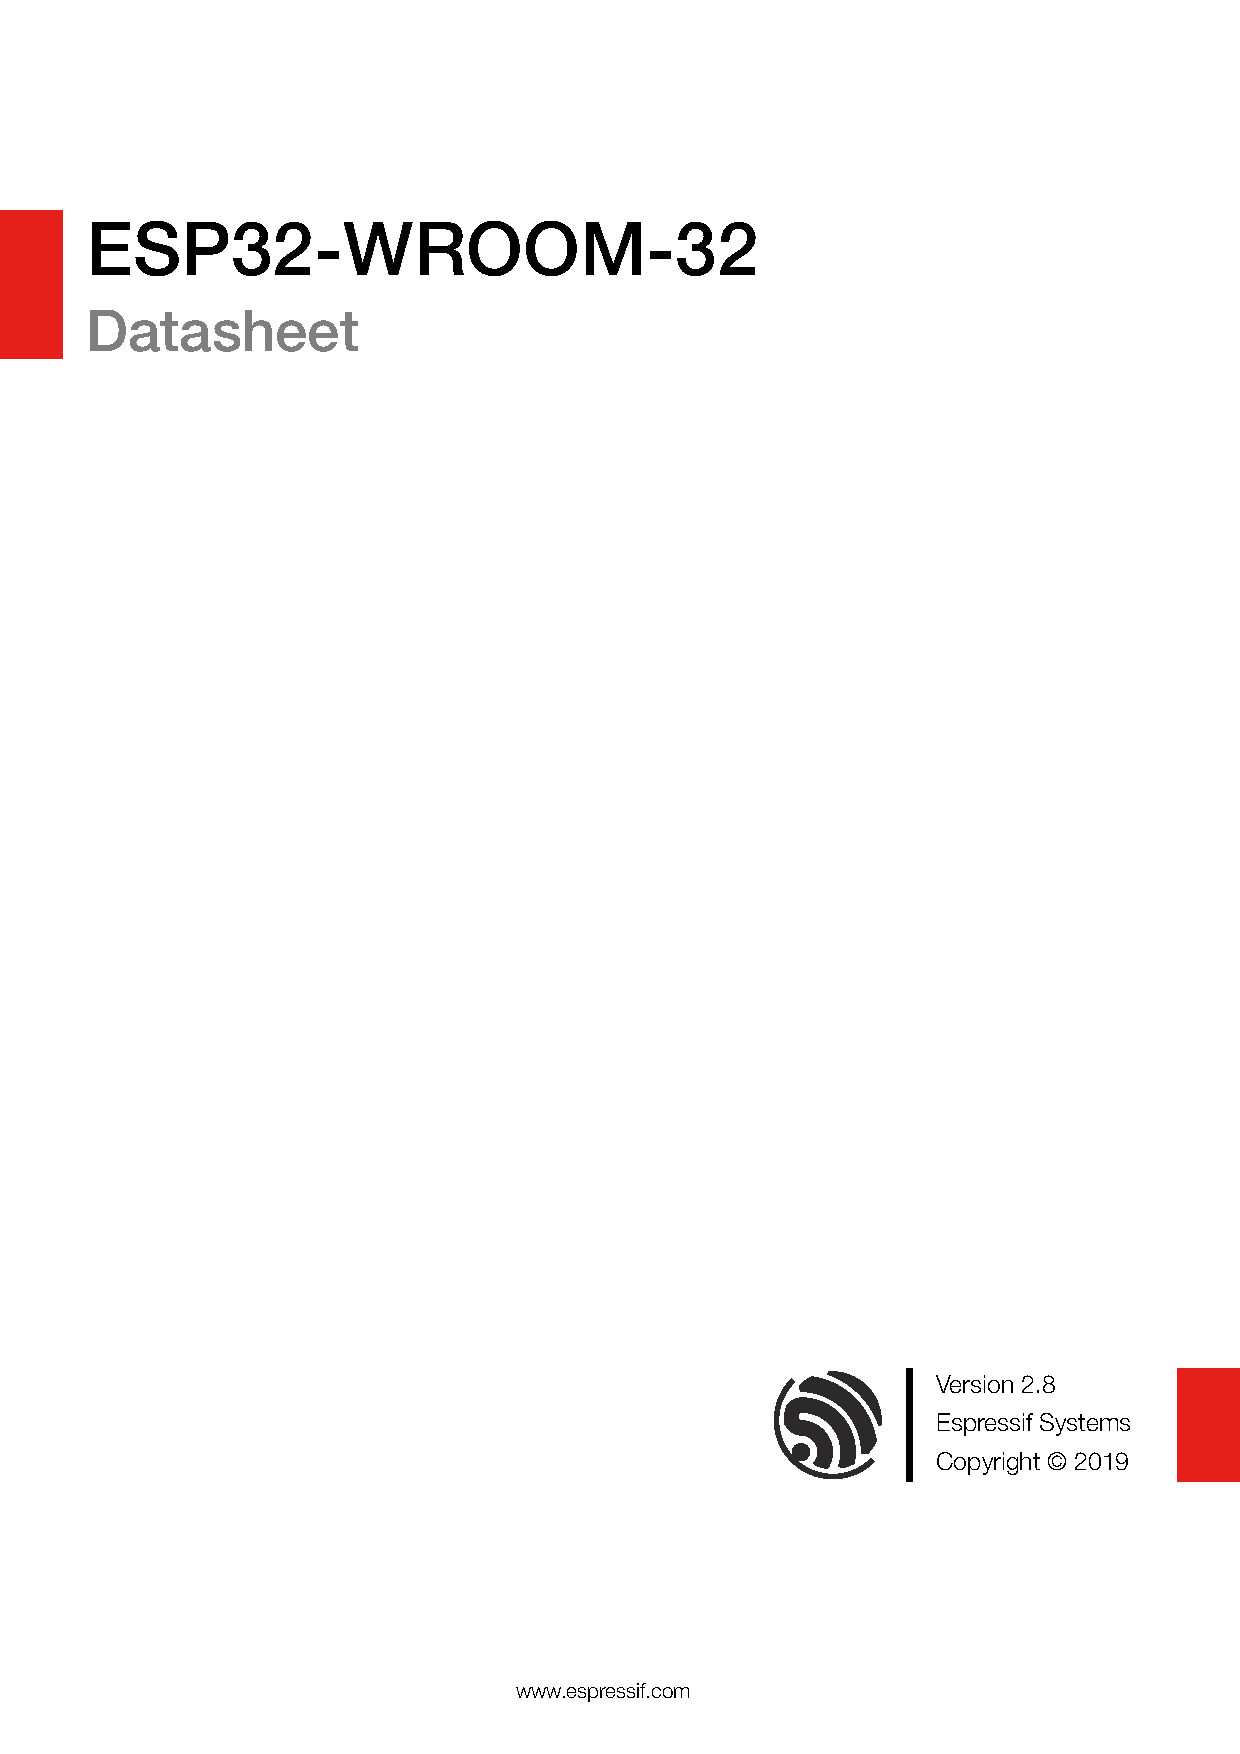
\includegraphics[height=0.75\textheight, frame]{esp32-wroom-32_datasheet_en.pdf}
    \caption{ESP32-WROOM-32 Datasheet (First Page)}
    \label{fig:esp-datasheet}
\end{figure}

\section{Appendix}
\subsection{Tables}
\begin{table}[H]
    \centering
    \begin{tabular}{|p{4cm} p{2cm} p{2cm} p{3cm} p{4cm}|}
        \hline
        \multicolumn{5}{|c|}{Statistical Inference Test of Unit Tests (268/268 assertions passed)} \\
        \hline
        Confidence Level (\%) & Z-Score & $\hat{p}$ & Standard Error & Confidence Interval \\
        \hline
        90 & 1.65  & 1 & 0 & 1 $\pm$ 0 \\
        95 & 1.96  & 1 & 0 & 1 $\pm$ 0 \\
        99 & 2.576 & 1 & 0 & 1 $\pm$ 0 \\
        \hline
    \end{tabular}
    \begin{tabular}{|p{4cm} p{2cm} p{2cm} p{3cm} p{4cm}|}
        \hline
        \multicolumn{5}{|c|}{Statistical Inference Test of Unit Tests (267/268 assertions passed)} \\
        \hline
        Confidence Level (\%) & Z-Score & $\hat{p}$ & Standard Error & Confidence Interval \\
        \hline
        90 & 1.65  & 0.9963 & 0.0002275 & 0.9963 $\pm$ 0.0003754 \\
        95 & 1.96  & 0.9963 & 0.0002275 & 0.9963 $\pm$ 0.0004459 \\
        99 & 2.576 & 0.9963 & 0.0002275 & 0.9963 $\pm$ 0.0005840 \\
        \hline
    \end{tabular}
    \begin{tabular}{|p{4cm} p{2cm} p{2cm} p{3cm} p{4cm}|}
        \hline
        \multicolumn{5}{|c|}{Statistical Inference Test of Unit Tests (258/268 assertions passed)} \\
        \hline
        Confidence Level (\%) & Z-Score & $\hat{p}$ & Standard Error & Confidence Interval \\
        \hline
        90 & 1.65  & 0.9627 & 0.01157 & 0.9627 $\pm$ 0.01910 \\
        95 & 1.96  & 0.9627 & 0.01157 & 0.9627 $\pm$ 0.02269 \\
        99 & 2.576 & 0.9627 & 0.01157 & 0.9627 $\pm$ 0.02982 \\
        \hline
    \end{tabular}
    \caption{Inference on Single Proportion Test Results. This shows that when all unit tests are passing, then there is a absolute confidence that the software will function correctly.}
    \label{tab:inference}
\end{table}

\begin{table}[H]
    \centering
    \begin{tabular}{|l|c c|c|}
        \hline
        \multicolumn{4}{|c|}{Microcontroller Code Coverage Report (LCOV)} \\
        \hline
        Measurement & Hit & Total & Coverage \\
        \hline
        Lines       & 100 & 100 & 100.0 \\
        Functions   & 28  & 28  & 100.0 \\
        \hline
    \end{tabular}
    \caption{Summary report of the locally generated coverage report using built-in gcc flags and lcov}
    \label{tab:covsummary}
\end{table}

\begin{table}[H]
    \centering
    \begin{tabular}{|l|c c|c c|}
        \hline
        \multicolumn{5}{|c|}{Microcontroller Code Coverage Report (LCOV)} \\
        \hline
        File & Line Coverage & Line Coverage (\%) & Functions & Functions (\%) \\
        \hline
        src/main.cpp                & 31/31 & 100.0 & 6/6   & 100.0 \\
        test/test\_main.cpp         & 54/54 & 100.0 & 7/7   & 100.0 \\
        test/mock/Arduino.h         & 3/3   & 100.0 & 3/3   & 100.0 \\
        test/mock/BluetoothSerial.h & 11/11 & 100.0 & 11/11 & 100.0 \\
        test/mock/Serial.h          & 1/1   & 100.0 & 1/1   & 100.0 \\
        \hline
    \end{tabular}
    \caption{Detailed report of the locally generated coverage report using built-in gcc flags and lcov}
    \label{tab:covdetailed}
\end{table}

\subsection{Figures}
\begin{figure}[H]
    \centering
    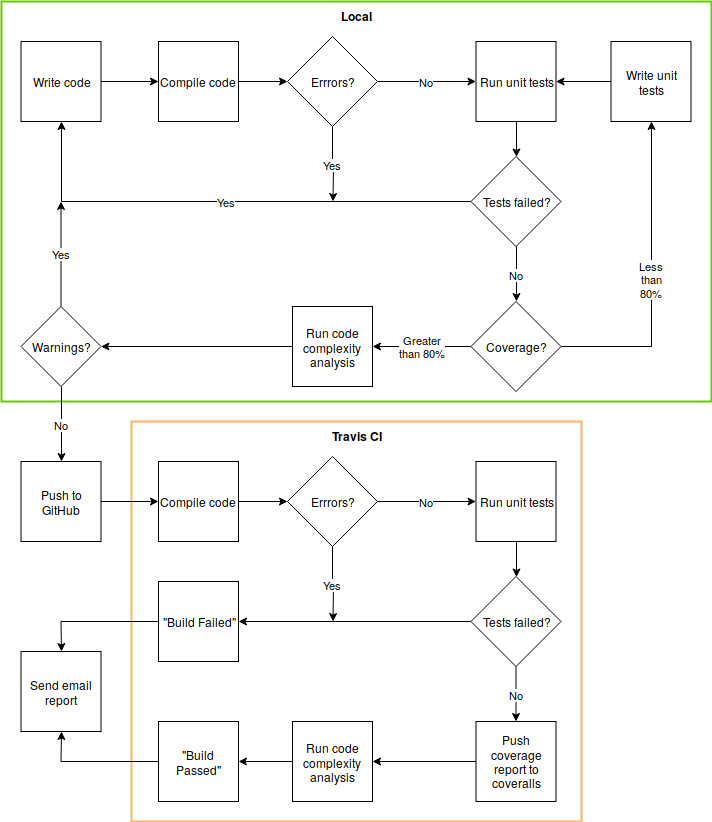
\includegraphics[scale=0.5]{images/workflow}
    \caption{The standard software testing workflow used for the microcontroller code. Note that a redundant process is run between the local code and the remote code on GitHub  through Travis CI.}
    \label{fig:workflow}
\end{figure}

\begin{figure}[H]
    \centering
    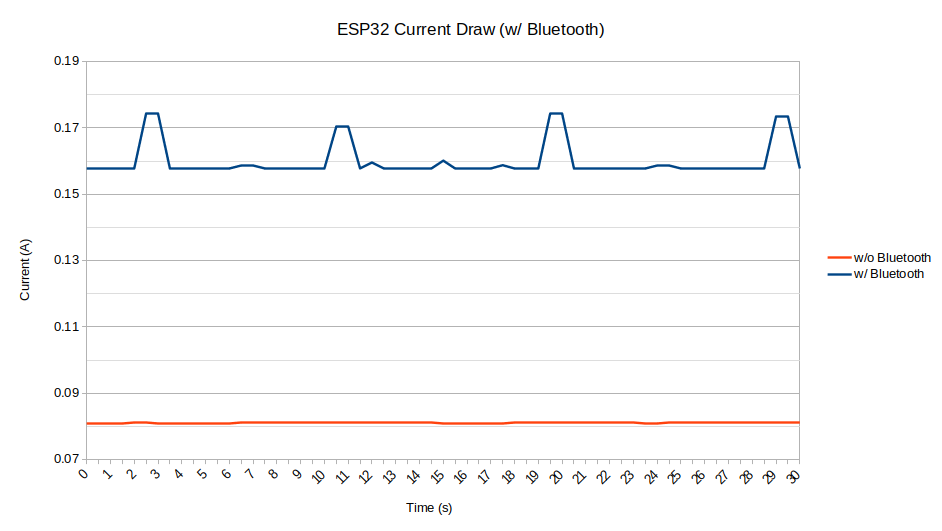
\includegraphics[scale=0.5]{images/powerdata}
    \caption{Measurement of current drawn by the microcontroller from a DC power supply. The consumption was first measured without an active Bluetooth connection, then again without an active connection. The peaks in current draw are most likely a periodic wake done by the Bluetooth controller to ensure that a connection stays established between devices.}
    \label{fig:powerdata}
\end{figure}

\begin{figure}[H]
    \centering
    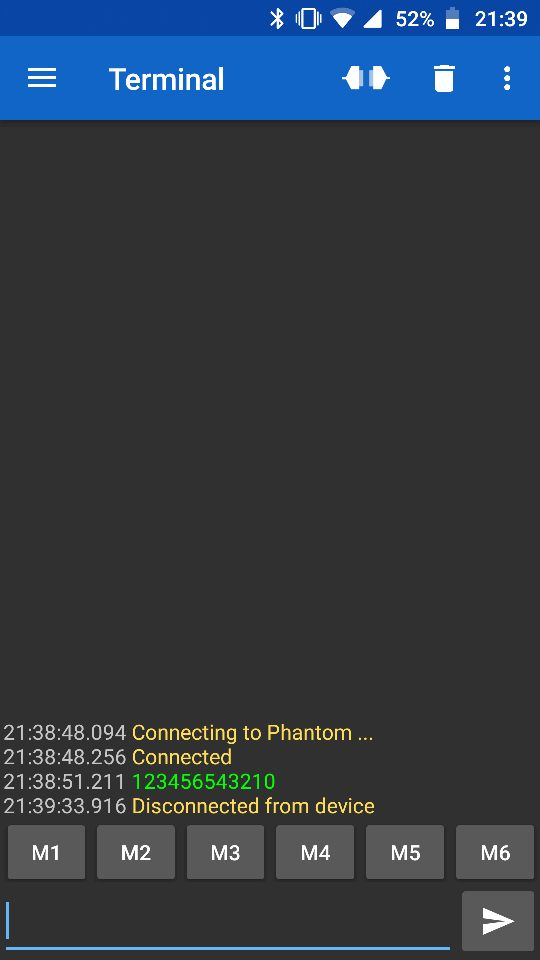
\includegraphics[scale=0.5]{images/functional}
    \caption{Functional test result for the microcontroller read using the Serial Bluetooth app available on the Google Play Store. Any serial terminal will also function though.}
    \label{fig:functional}
\end{figure}

\subsection{Unit Test Code Example}
\lstinputlisting[language=C++]
{code/test.cpp}

\subsection{Code Complexity Report}
\lstinputlisting
{code/complexity.txt}

\subsection{Links}
Travis CI: https://travis-ci.org/omn0mn0m/Balloon-Catheterization/

Coveralls: https://coveralls.io/github/omn0mn0m/Balloon-Catheterization

\section{Revision History}
\begin{versionhistory}
  \vhEntry{1.0}{04/10/2019}{NT}{Original Draft}
  \vhEntry{1.0}{04/28/2019}{NT}{Original Release}
  \vhEntry{1.0}{04/29/2019}{NT}{Edit to include more details}
\end{versionhistory}

\end{document}
